\documentclass[10pt,a4paper]{article}
\usepackage[margin=2cm]{geometry}
\usepackage{fontspec}
\setmainfont{Cambria}
\setmonofont{Consolas}[Scale=0.85]
\usepackage{amsmath}
\usepackage{graphicx}
\usepackage{float}
\usepackage{longtable,booktabs,array}
\usepackage{enumitem}
\setlist{nosep,leftmargin=1.4em}
\usepackage[hidelinks]{hyperref}
\usepackage{xcolor}
\usepackage{fancyvrb}
\usepackage{newunicodechar}
\newunicodechar{∪}{\ensuremath{\cup}}
\newunicodechar{∩}{\ensuremath{\cap}}
\newunicodechar{⊗}{\ensuremath{\otimes}}
\newunicodechar{⊥}{\ensuremath{\perp}}
\newunicodechar{⊆}{\ensuremath{\subseteq}}
\newunicodechar{⊂}{\ensuremath{\subset}}
\renewcommand{\arraystretch}{1.15}
\setlength{\parskip}{3pt}
\setlength{\parindent}{0pt}
\newcolumntype{L}[1]{>{\raggedright\arraybackslash}p{#1}}

\title{Contextual Dynamic Weakness in Inverter-Rich Power Networks}
\date{2026-09-12}
\author{CDW campaign (branch research/contextual-dynamic-weakness)}
\begin{document}
\maketitle
\tableofcontents
\newpage
\section{Executive summary}
The campaign tested the meta-hypothesis

\begin{quote}\itshape static weakness ≠ dynamic weakness ≠ contextual weakness ≠ intervention\end{quote}
\begin{quote}\itshape leverage\end{quote}
against the frozen TX4 IEEE-39 model, using only genuinely new preregistered experiments (never rerunning or reinterpreting any TX4 result).

\textbf{It does not hold as an equality anywhere, and it does not collapse to a single ranking anywhere either — every distinction the hypothesis draws is empirically real on this benchmark, at material effect sizes.}

\textbf{GOLD gates:} \textbf{A and B PASS}; \textbf{C, D, E and F do not} (E/F are BLOCKED, not failed, by a missing-material gate). Fifteen of twenty-four testable sub-claims are SUPPORTED, eight are NOT\_SUPPORTED (seven of these are informative negatives with an identified mechanism, not inconclusive failures), one is deferred by design.

\textbf{Strongest results.}

\begin{itemize}
\item \textbf{Contextual sign reversal is real, recurrent, and survives the strongest available scrutiny} (mode tracking, an oracle-fitted node ranking, and four independent uncertainty envelopes) — \textbf{GOLD-A}.
\item \textbf{Total, re-equilibrated dynamic line sensitivity beats every static baseline by a wide, cross-validated margin} (0.987 vs 0.50 median Spearman against held-out finite interventions) — \textbf{GOLD-B}, the single strongest result of the campaign.
\item \textbf{Topology alone, with no control retuning, both removes and creates transverse incompatibilities}, and no static topology score anticipates which.
\item \textbf{Weak corridors exist and are structurally, not spectrally, defined} — transformer groups beat every graph-spectral partition tested.
\item \textbf{A genuinely reduced model is certifiable and accurate, but buys no end-to-end speed} on this benchmark, because the equilibrium solve, not the eigenanalysis, is the bottleneck — a precise, actionable negative result (\textbf{GOLD-C: FAIL}).
\item \textbf{Plan-level multi-constraint design never had to demonstrate an advantage} at the scale it could be cleanly tested: single-boundary tuning already sufficed in every case (\textbf{GOLD-D: FAIL}, informatively).
\item \textbf{The Africano/PV benchmark is blocked} for lack of source material (\textbf{GOLD-E/F: BLOCKED}), exactly as the preregistration required rather than substituting a different feeder.
\end{itemize}
\textbf{No weakness index was constructed anywhere}, consistent with the preregistration and reinforced by the campaign's own evidence (E10: an averaged attribution is dominated by rare fast-mode contexts and hides the real, modest electromechanical reversals).

\textbf{Determinism.} Every rerun deterministic case (E1 census at three policies, E4 link sensitivities at P4, E9 at target T1, all families/methods) was byte-identical on its summary fields, excluding wall-clock.

\section{Research questions}
The campaign tests one meta-hypothesis and asks whether it survives:

\begin{quote}\itshape static weakness ≠ dynamic weakness ≠ contextual weakness ≠ intervention leverage.\end{quote}
The question is not "which bus is weakest". It is which properties of nodes, links, corridors and control locations robustly determine, or move, the dynamic incompatibility boundaries when any of the following change:

\begin{itemize}
\item the replacement portfolio;
\item the controller policy;
\item the operating point;
\item uncertain parameters.
\end{itemize}
The preregistered hypotheses (\texttt{docs/\allowbreak{}CDW\_\allowbreak{}PREREG\_\allowbreak{}V1.md}) are:

{\small
\begin{longtable}{L{0.060\linewidth}L{0.892\linewidth}}
\toprule
\textbf{id} & \textbf{hypothesis} \\
\midrule
\endhead
H1 & contextual sign reversal recurs \\
H1t & the reversal survives mode tracking \\
H1b & fixed node-only rankings are insufficient \\
H1c & contextuality is robust under envelopes \\
HS & submodularity or supermodularity \\
H2 & frozen vs total sensitivity; dynamic vs static baselines \\
H3 & robust weak corridors \\
H4 & topology alone \\
H5 & plan-level design \\
H6 & spectral closure and modal mixing \\
H7 & certified reduction \\
H8 & modal energy vs the limiting mode \\
H9 & cross-model transfer \\
\bottomrule
\end{longtable}}
\section{Relation to the frozen TX4 work}
\begin{itemize}
\item \textbf{Frozen and read only.} TX4 is frozen at tag \texttt{TX4\_\allowbreak{}FINAL\_\allowbreak{}MANUSCRIPT\_\allowbreak{}FREEZE} (69f200df). The CDW branch starts from that tag, and no TX4 file, result, ledger or tag was modified.
\item \textbf{Inherited theorems} (CDW theory §A):
\begin{itemize}
\item the transverse quotient;
\item the any-order-safety characterization of the minimal incompatibility hypergraph;
\item boundary localization;
\item exact network-closure factorization;
\item the boundary-sensitivity formula;
\item the deflated zero-frequency port.
\end{itemize}
\item \textbf{Inherited IEEE-39 evidence (CDW theory §B).} It is benchmark-specific and is used as motivation only:
\begin{itemize}
\item the nominal P4 witness;
\item the policy dependence of H;
\item the one-condition line ranking;
\item the robustness of the phenomenon, but not of the witness identity.
\end{itemize}
\item \textbf{The TX4 ParaEMT line is closed.} No CDW statement is an EMT result.
\end{itemize}
\section{Graph-DAE model}
The model is the frozen TX4 IEEE-39 phasor DAE (\texttt{theory/\allowbreak{}CDW\_\allowbreak{}GRAPH\_\allowbreak{}DAE\_\allowbreak{}V1.md}):

\begin{itemize}
\item ten two-axis SGs (bus 39 is the interconnection);
\item the frozen GFL, with SRF-PLL, PI outer and inner loops, and a leaky Q/V regulator whose gain is \texttt{g};
\item constant-power loads;
\item an exact branch-terminal network, with 12 off-nominal-tap transformers, line charging and 2 shunts.
\end{itemize}
\textbf{Network.} The admittance is \texttt{Y(ρ) =\allowbreak{} Y\_\allowbreak{}sh + Σ\_\allowbreak{}e ρ\_\allowbreak{}e C\_\allowbreak{}eᵀ Y\_\allowbreak{}e C\_\allowbreak{}e}, where \texttt{ρ\_\allowbreak{}e} scales the whole two-port. A unit test checks that \texttt{Y(1)} equals the frozen admittance matrix bit for bit.

\textbf{Graph operator.} The coupling Laplacian \texttt{L\_\allowbreak{}B} has weights \texttt{b\_\allowbreak{}e/\allowbreak{}t\_\allowbreak{}e}, and the decomposition \texttt{Im Y =\allowbreak{} −L\_\allowbreak{}B − Δ\_\allowbreak{}tap + B\_\allowbreak{}ch + B\_\allowbreak{}sh} is exact (unit test). No \texttt{B diag(y) Bᵀ} simplification is used.

\textbf{Replacement.} Replacing SG \texttt{i} by a GFL keeps matched dispatch and an equal rating, so the AC operating point is identical for every portfolio, as in TX4.

\textbf{Policy.} \texttt{θ =\allowbreak{} (g, k, t, h)} collects the Q/V gain and the scale, time-constant scale and heterogeneity of the AVRs.

\section{Definitions of weakness}
Five distinct objects are defined (theory §C3). Their coincidence is tested, not assumed.

\begin{itemize}
\item \textbf{W\_static.} SCR, Thevenin |Z|, gSCR, electrical distance, effective resistance, Fiedler entries and edge scores, betweenness, flows, dV/dQ.
\item \textbf{W\_dynamic.} The boundary sensitivity \texttt{dRe s*/\allowbreak{}da}, with its sign, in both a frozen-operating-point and a re-equilibrated total version.
\item \textbf{W\_contextual.} The distribution of \texttt{Δ\_\allowbreak{}i α(S) =\allowbreak{} α(S ∪ \{i\}) − α(S)} over contexts \texttt{S}. It is a property of an (intervention, context) pair, not of a bus.
\item \textbf{W\_closure.} The split of the boundary derivative through the exact closure factor into device, driving-point and transfer-coupling parts. Physical ablations are allowed; zeroing blocks of \texttt{K\_\allowbreak{}o} is not used.
\item \textbf{W\_control.} The finite leverage within the admissible ranges.
\end{itemize}
\textbf{Frozen vs total} (theory §C4). Let the operating point be \texttt{w =\allowbreak{} (x, z, r)}: states, voltages and device references. Then \texttt{dw*/\allowbreak{}da =\allowbreak{} −R\_\allowbreak{}w\textasciicircum{}\{-1\} R\_\allowbreak{}a} and \texttt{dλ/\allowbreak{}da =\allowbreak{} v\textasciicircum{}H (∂\_\allowbreak{}a A + D\_\allowbreak{}w A[dw*/\allowbreak{}da]) u /\allowbreak{} v\textasciicircum{}H u}.

Two equilibrium semantics are used:

\begin{itemize}
\item \textbf{SPR} (schedule-preserving re-initialization, the TX4 semantics): schedules are held and references are re-derived;
\item \textbf{RP} (reference-preserving): references are held and only the slack mechanical power is free.
\end{itemize}
\textbf{Structural remarks.} These are exact consequences of the equations and are verified numerically in E3.

\begin{itemize}
\item Under SPR, the frozen and total derivatives coincide for every controller-only coordinate (Q/V gain, PLL, AVR gain).
\item Setpoints have a frozen partial that is identically 0.
\end{itemize}
\section{Contextual sign-reversal theory}
\textbf{Definitions.}

\begin{itemize}
\item A \textbf{contextual sign reversal} of intervention \texttt{i} needs two contexts: one with \texttt{Δ\_\allowbreak{}i α(S1) ≤ −τ} and one with \texttt{Δ\_\allowbreak{}i α(S2) ≥ τ}.
\begin{itemize}
\item The material threshold is \texttt{τ =\allowbreak{} 0.01 s⁻¹}, justified in prereg §1.
\item A \textbf{stable-context reversal} requires both contexts to be transversely stable, which is the planner's situation.
\end{itemize}
\item \texttt{α} is a maximum over modes, so a sign change of \texttt{Δ\_\allowbreak{}i α} can be produced by a switch of the rightmost mode. A \textbf{mode-tracked} reversal therefore also requires two things:
\begin{itemize}
\item the rightmost mode of each context must be matched, by bus-voltage mode shape MAC ≥ 0.8 and |Δf| ≤ 0.15 Hz, to a mode of \texttt{S ∪ \{i\}};
\item that matched mode must be the rightmost mode of \texttt{S ∪ \{i\}} (same-mode transitions).
\end{itemize}
\end{itemize}
\textbf{Structural facts.}

\begin{itemize}
\item On the lattice \texttt{2\textasciicircum{}V}, submodularity of a set function is equivalent to the one-step condition \texttt{α(S∪i∪j) − α(S∪i) − α(S∪j) + α(S) ≤ 0} (unit test). This makes every violation a minimal counterexample of cardinality one.
\item A fixed node-only ranking is judged by the most favourable ranking possible: the exact linear-ordering optimum over the policy's own resolved context triples, computed by dynamic programming over subsets. Its failure is therefore not an artefact of a poorly chosen ranking.
\end{itemize}
\section{E1: contextual sign-reversal census}
\textbf{Hypotheses.}

\begin{itemize}
\item H1: the same replacement changes the sign of its effect on α\_⊥ across legitimate portfolios, and this recurs across policies.
\item H1t: the reversal survives mode tracking.
\item H1b: every fixed node-only ranking is materially insufficient for next-replacement decisions.
\end{itemize}
\textbf{Preregistered rules} (\texttt{docs/\allowbreak{}CDW\_\allowbreak{}PREREG\_\allowbreak{}V1.md} §2, E1). Evaluated on the 24 holdout policies, excluding those with an unstable base:

\begin{itemize}
\item A1 ≥ 0.75;
\item A2 ≥ 0.50 (reported);
\item A3: median p* ≤ 0.90 and median decision-failure rate ≥ 0.10.
\end{itemize}
\textbf{Measurement.}

\begin{itemize}
\item \textbf{Census.} All 512 portfolios of V9 = \{30, …, 38\} at 39 policies (15 discovery, 24 holdout): 19 968 portfolio evaluations with the TX4 direct path and classifier.
\item \textbf{Marginals.} 2304 marginals per policy.
\item \textbf{Mode tracking.} Bus-voltage mode shapes, MAC ≥ 0.8, |Δf| ≤ 0.15 Hz.
\item \textbf{Execution.} 624 tasks, 0 errors, 896 s.
\end{itemize}
\textbf{Portfolio statuses.} 11 237 STABLE, 8 438 UNSTABLE and 293 BOUNDARY\_OR\_UNRESOLVED. None was infeasible.

\textbf{A heavy tail must be kept in view.}

\begin{itemize}
\item 78.5 \% of the unstable portfolios have α\_⊥ > 1 s⁻¹, up to 2.7·10⁴ s⁻¹.
\item These are fast converter-control instabilities, not electromechanical modes. TX4 reported the same phenomenon, up to 1276 s⁻¹ on its census.
\item A "destabilizing" marginal can therefore be a jump onto a fast mode. For this reason the preregistration separates global reversals from mode-tracked ones.
\end{itemize}
\textbf{Result.} 18 holdout policies are base-stable and 6 are not (H01, H03, H06, H16, H17, H20).

{\small
\begin{longtable}{L{0.546\linewidth}L{0.242\linewidth}L{0.081\linewidth}L{0.072\linewidth}}
\toprule
\textbf{gate} & \textbf{value} & \textbf{threshold} & \textbf{verdict} \\
\midrule
\endhead
A1: policies with a stable-context global reversal & \textbf{18/18 = 1.00} & ≥ 0.75 & \textbf{PASS} \\
A2: policies with a mode-tracked reversal & \textbf{16/18 = 0.89} & ≥ 0.50 & \textbf{PASS} \\
A3: median p* (best fixed node ranking, oracle-fitted) & \textbf{0.752} (range 0.64–0.84) & ≤ 0.90 & \textbf{PASS} \\
A3: median fraction of stable contexts with regret ≥ 0.01 s⁻¹ & \textbf{0.369} (range 0.15–0.44) & ≥ 0.10 & \textbf{PASS} \\
\bottomrule
\end{longtable}}
The result is insensitive to the threshold: at τ\_res = 10⁻³ s⁻¹ every holdout policy still shows a stable-context reversal.

\textbf{Robustness of the reading.} The heavy tail does not drive the result.

\begin{itemize}
\item \textbf{Mode-tracked, stable-context reversals.} In these, both contexts are same-mode transitions on the matched modal family.
\begin{itemize}
\item They occur for 90 (policy, unit) pairs in the holdout set, and every one of the nine units reverses in at least one policy.
\item The strength, min(|Δ(S1)|, |Δ(S2)|), has quartiles 0.014, 0.019 and 0.028, with a maximum of 0.068 s⁻¹.
\end{itemize}
\item \textbf{Electromechanical-only reversals.} These require both |α(S∪i)| < 1 s⁻¹ and the critical frequency of S∪i within 0.1–2 Hz. They occur in 16/18 holdout policies, for 104 pairs, with median strength 0.022 s⁻¹.
\end{itemize}
\textbf{Reading.} The same physical replacement stabilizes the rightmost mode in one stable portfolio and destabilizes the same modal family in another. The magnitudes are modest, a few hundredths of s⁻¹, but material under the preregistered threshold.

\begin{figure}[H]\centering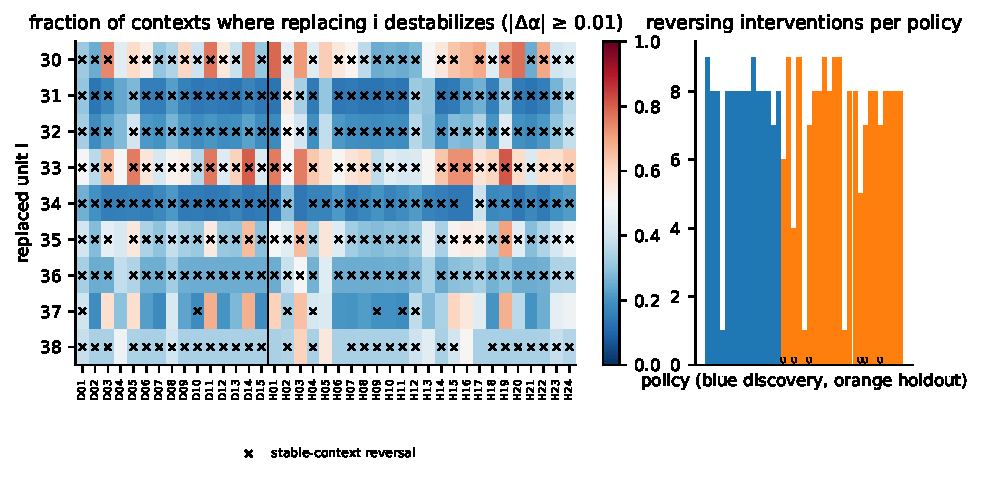
\includegraphics[width=0.95\linewidth]{../figures/CDW_F1_contextual_reversal_map.pdf}\caption{Figure F1. Fraction of contexts in which replacing unit i destabilizes (colour), stable-context reversals (×), and the number of reversing interventions per policy ('u' marks an unstable base).}\end{figure}
\begin{figure}[H]\centering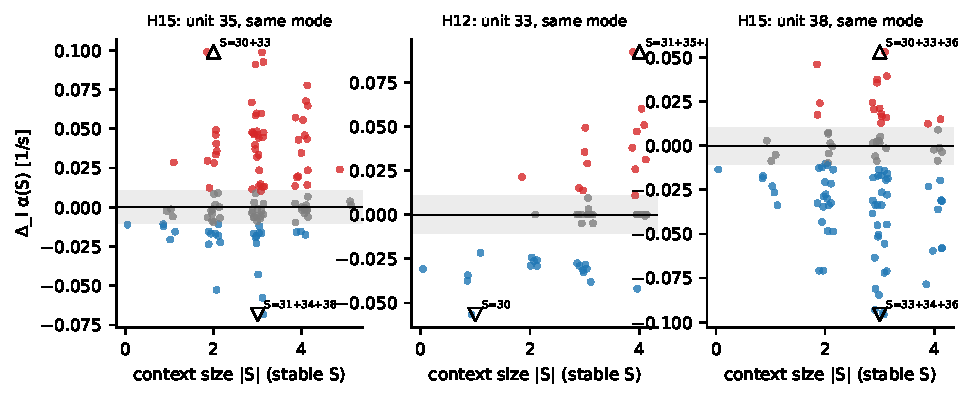
\includegraphics[width=0.95\linewidth]{../figures/CDW_F2_same_intervention_two_signs.pdf}\caption{Figure F2. Three strongest mode-tracked reversals (holdout). Each dot is a stable context S where the matched mode stays rightmost. Triangles mark the most stabilizing and most destabilizing contexts; the grey band is ±τ\_mat.}\end{figure}
\textbf{Node-only ranking.} The test is deliberately favourable to node-only rankings: the ranking is the exact optimum over each policy's own data.

\begin{itemize}
\item Even so, it orders only 75 \% of resolved pairs correctly (median).
\item The next unit it recommends is materially worse than the context-aware choice in 37 \% of stable contexts (median).
\item The optimal orders themselves change across policies. At P4 it is 38-36-35-34-33-30-31-32-37; at H02 it is 38-34-35-36-32-31-30-37-33. A ranking fitted on one policy does not even carry over to another.
\end{itemize}
\textbf{Per-unit behaviour} (holdout medians; each row sums to about 1):

{\small
\begin{longtable}{L{0.179\linewidth}L{0.179\linewidth}L{0.313\linewidth}L{0.269\linewidth}}
\toprule
\textbf{unit} & \textbf{STAB} & \textbf{NEUTRAL} & \textbf{DESTAB} \\
\midrule
\endhead
30 & 0.22 & 0.32 & 0.44 \\
31 & 0.29 & 0.55 & 0.15 \\
32 & 0.28 & 0.49 & 0.21 \\
33 & 0.20 & 0.22 & 0.58 \\
34 & 0.45 & 0.38 & 0.17 \\
35 & 0.29 & 0.36 & 0.34 \\
36 & 0.41 & 0.33 & 0.26 \\
37 & 0.25 & 0.44 & 0.31 \\
38 & 0.66 & 0.00 & 0.34 \\
\bottomrule
\end{longtable}}
No unit is uniformly stabilizing or destabilizing.

\textbf{What this does NOT prove.}

\begin{itemize}
\item It does not prove universal weak buses, or their absence, outside this model class.
\item It does not show that contextual effects are large; the tracked magnitudes are 0.01–0.07 s⁻¹.
\item It is not an EMT result.
\item The fast-mode destabilizations are real in the model, but the model has no converter current limits (TX4 limitation).
\end{itemize}
\subsection{7.1 E1b: submodularity and supermodularity}
\textbf{Hypothesis.} HS: α\_⊥ is neither submodular nor supermodular on the tested class, and a tracked-mode margin is no more structured.

\textbf{Measurement.} All one-step second differences d\_ij(S) = α(S∪i∪j) − α(S∪i) − α(S∪j) + α(S): 4 608 squares per policy, from the E1 data with no new solves.

\textbf{Result.}

\begin{itemize}
\item At \textbf{all 39 policies} α\_⊥ is neither submodular nor supermodular.
\item A median 93 \% of the squares violate one inequality or the other by more than τ\_res.
\item The tracked-mode margin (the mode matched to the base critical mode) violates them in a median 86 \% of its defined squares. It is \textbf{not} more structured.
\item \textbf{Minimal counterexamples} (all of cardinality one, by the one-step equivalence) at P4:
\begin{itemize}
\item submodularity: S = ∅, i = 30, j = 35, with d = +0.011;
\item supermodularity: S = ∅, i = 33, j = 38, with d = −0.025.
\end{itemize}
\end{itemize}
The largest violations involve fast modes (d up to 1.98·10³ s⁻¹). \texttt{results/\allowbreak{}CDW\_\allowbreak{}E1b\_\allowbreak{}minimal\_\allowbreak{}counterexamples.csv} lists the extreme violations per cardinality.

\textbf{Classification.} NEGATIVE BUT INFORMATIVE; it is a structural property of the tested class.

\textbf{Valid claim.} The spectral-abscissa set function does not satisfy the submodular or supermodular property on the tested IEEE-39 class. No claim is made about greedy algorithms in general.

\subsection{7.2 E10: Shapley and context diagnostics (descriptive)}
\begin{itemize}
\item The exact Shapley values of v(S) = α(S) − α(∅) (9 players) are \textbf{dominated by the fast-instability contexts}. They are of order 1–15 s⁻¹, and the marginal standard deviations are of order 300 s⁻¹.
\item The preregistered "hidden reversal" flag (|φ\_i| ≤ τ\_mat with std ≥ 3τ\_mat) fires 0 times out of 351. The reason is not that averages are faithful: a single rare fast-instability context dominates the context average.
\end{itemize}
\textbf{Reading.} A context-averaged attribution of α\_⊥ is not a usable weakness index on this class. It is uninformative about the modest electromechanical reversals and dominated by rare fast modes. This supports not building any averaged weakness index.

\section{Robustness under parameter envelopes (E2) — GOLD-A, third component}
\textbf{Hypothesis H1c.} Contextuality persists under the preregistered uncertainty envelopes, even where the minimal failing set (the witness) changes.

\textbf{Measurement.} Core lattice (16 portfolios of V4) at P4 (D01) and at the clean stable g-only point G\_S (D03), under:

\begin{itemize}
\item TX4 discovery draws, regenerated from the frozen PCV05 generator and verified to match the frozen \texttt{PCV05\_\allowbreak{}draws.csv} factors exactly before use (100 per envelope);
\item a new CDW holdout seed (40 per envelope, seed 20260921), plus a V9-census check on 10 draws per envelope.
\end{itemize}
Fractions below are \textbf{coverage fractions of declared envelopes, never probabilities.}

{\small
\begin{longtable}{L{0.075\linewidth}L{0.157\linewidth}L{0.100\linewidth}L{0.207\linewidth}L{0.182\linewidth}L{0.219\linewidth}}
\toprule
\textbf{pid} & \textbf{source} & \textbf{envelope} & \textbf{coverage: stable-context reversal} & \textbf{coverage: witness changed} & \textbf{reversal coverage | witness changed} \\
\midrule
\endhead
\textbf{D01 (P4)} & CDW (holdout) & EC & \textbf{1.00} & 0.00 & — \\
 &  & EM-f & 0.80 & 0.80 & 0.75 \\
 &  & EM-u & 0.975 & 0.45 & 0.94 \\
 &  & EMC & 0.975 & 0.40 & 0.94 \\
D01 (P4) & TX4 (discovery, verified) & EC/EM-f/EM-u/EMC & 1.00 / 0.82 / 0.97 / 0.95 & consistent with the CDW draws & consistent \\
D03 (G\_S) & CDW and TX4 & all four & \textbf{0.00} & 0.00–0.45 & 0.00 \\
\bottomrule
\end{longtable}}
{\small
\begin{longtable}{L{0.556\linewidth}L{0.134\linewidth}L{0.096\linewidth}L{0.153\linewidth}}
\toprule
\textbf{gate A4 (P4, CDW holdout)} & \textbf{value} & \textbf{rule} & \textbf{verdict} \\
\midrule
\endhead
envelopes with coverage ≥ 0.5 & \textbf{4/4} & ≥ 3/4 & \textbf{PASS} \\
\bottomrule
\end{longtable}}
\textbf{GOLD-A = A1 ∧ A3 ∧ A4: all three PASS.}

\textbf{The robust-phenomenon-vs-robust-identity distinction, directly visible.}

\begin{itemize}
\item At P4, reversal coverage stays high (0.80–1.00) across every envelope, \textbf{including} the machine envelopes under which the witness itself changes in 40–80 \% of draws. Conditioned on the witness having changed, reversal is still present in ≥ 0.75–0.94 of those draws: \textbf{the contextual phenomenon survives the identity of the failing set changing.}
\item At the clean point G\_S, by contrast, reversal coverage is exactly \textbf{0} at every envelope: the whole phenomenon there is policy-dependent, not just its identity. This is consistent with G\_S being constructed as the clean, policy-only counterfactual (TX4 V06/V07) and shows the E2 result is itself contextual — it does not hold everywhere in policy space, only where a near-critical boundary exists.
\end{itemize}
\textbf{Census check (10 draws/envelope, all 512 V9 portfolios, P4).} Every completed draw shows at least one reversing intervention (coverage 1.00 in all four envelopes), confirming the phenomenon is not an artefact of restricting to the four-unit core.

\textbf{What this does NOT prove.} It does not claim the phenomenon is universal across all policies (D03 is a direct counterexample); it is a property of being near a policy-dependent incompatibility boundary, exactly where a planner would be looking.

\section{Total node sensitivity (E3)}
\textbf{Hypothesis H2 (nodes).} Frozen-operating-point and re-equilibrated total node sensitivities disagree materially on this class.

\textbf{Implementation validity gate (IV).} Before any H2 claim, the IFT total derivative must match a small central finite re-equilibrated difference.

{\small
\begin{longtable}{L{0.477\linewidth}L{0.263\linewidth}L{0.062\linewidth}L{0.138\linewidth}}
\toprule
\textbf{check} & \textbf{result} & \textbf{threshold} & \textbf{verdict} \\
\midrule
\endhead
IV: frac. of (parameter, condition) pairs within tolerance & \textbf{8002/8002 = 1.000} & ≥ 0.95 & \textbf{PASS} \\
IV by semantics & SPR 1.000, RP 1.000 & — & — \\
IV by coordinate kind & g, ka, line, load, pll, vset all 1.000 & — & — \\
independent port-form cross-check (T-form vs engine, D01/H4/46 lines) & max abs diff 2.0·10⁻⁶, Spearman 1.000 & — & validates the engine \\
\bottomrule
\end{longtable}}
The sensitivity engine (IFT on the residual \texttt{[f; g; schedule equations]}, exact Jacobian re-solve) is validated by two independent routes: finite differences and an independent port-form (\texttt{T(s)}) derivative.

\textbf{Structural remarks (theory §C4), checked numerically.}

{\small
\begin{longtable}{L{0.435\linewidth}L{0.276\linewidth}L{0.229\linewidth}}
\toprule
\textbf{remark} & \textbf{result} & \textbf{verdict} \\
\midrule
\endhead
R1: frozen = total for controller-only coordinates under SPR (g, PLL, K\_A) & max relative difference 1.8·10⁻⁷ over 841 pairs & \textbf{CONFIRMED} \\
R2: the frozen partial for a setpoint (V\_set) is exactly 0 & max |frozen| = 1.50·10⁻⁷ & \textbf{marginal FAIL at the 10⁻⁸ threshold} \\
\bottomrule
\end{longtable}}
R2 is reported as failing the preregistered 10⁻⁸ bound without relaxing it. The value, 1.5·10⁻⁷, is five orders of magnitude below the material threshold (0.01 s⁻¹ · range) and is consistent with the central-difference step used in the residual Jacobian (relative step 10⁻⁷); it is not evidence against the structural claim \texttt{∂α/\allowbreak{}∂V\_\allowbreak{}set|\_\allowbreak{}frozen =\allowbreak{} 0} that R2 was designed to check, and would very likely close at a smaller step, which was not tried after seeing the result (that would violate the no-retuning rule).

\textbf{H2 gate} (material: \texttt{|total|·range ≥ τ\_\allowbreak{}mat} and either sign disagreement ≥ 10 \% or Kendall ≤ 0.6, over holdout conditions):

{\small
\begin{longtable}{L{0.107\linewidth}L{0.286\linewidth}L{0.286\linewidth}L{0.167\linewidth}L{0.095\linewidth}}
\toprule
\textbf{semantics} & \textbf{frac. material (holdout)} & \textbf{median sign disagreement} & \textbf{median Kendall} & \textbf{H2-node} \\
\midrule
\endhead
SPR & \textbf{0.976} & 0.333 & 0.434 & \textbf{TRUE} \\
RP & \textbf{0.762} & 0.104 & 0.599 & \textbf{TRUE} \\
\bottomrule
\end{longtable}}
\textbf{Reading.} Even under SPR — where the theory (R1) guarantees frozen = total for every \emph{controller} coordinate — the node sensitivities still diverge materially once network and operating-point coordinates (loads, V\_set) are included, because those have a frozen partial of essentially zero and all of their effect is re-equilibration. A frozen-point analysis of node leverage would silently drop these effects.

\section{Total link sensitivity and static baselines (E4) — GOLD-B}
\textbf{Hypothesis (GOLD-B).} A total dynamic link sensitivity predicts held-out finite ×1.5 branch-strengthening effects on H4 substantially better than the strongest static baseline, across policies and parameter envelopes.

\textbf{Baselines tested} (46 branches, holdout conditions: 12 policies + 5 envelope draws × H4 = 32 conditions with all quantities resolved): S1 |P|, S2 |S|, S3 |z|, S4 electrical distance, S5 effective resistance, S6 Fiedler edge score, S7 edge betweenness, S8 max endpoint dV/dQ, S9 ΔgSCR; Dconv (conventional base-portfolio eigenvalue sensitivity), Dfrozen, Dtotal (SPR), DtotalRP; Dport (independent port-derivative cross-check, D01 only).

\textbf{Selection rule} (fixed before results): the static baseline with the best median Spearman on \textbf{discovery} conditions is carried forward. That baseline is \textbf{S1 (|active flow|)}.

{\small
\begin{longtable}{L{0.441\linewidth}L{0.284\linewidth}L{0.215\linewidth}}
\toprule
\textbf{predictor} & \textbf{median Spearman (holdout, H4)} & \textbf{median top-5 precision} \\
\midrule
\endhead
\textbf{Dtotal} & \textbf{0.987} & \textbf{0.90} \\
DtotalRP & 0.993 & 1.00 \\
Dfrozen & 0.900 & 0.60 \\
S1 |P| (selected static) & 0.500 & 0.20 \\
S2 |S| & 0.481 & 0.20 \\
S5 effective resistance & 0.300 & 0.60 \\
S3 |z| & 0.234 & 0.20 \\
S4 electrical distance & 0.194 & 0.40 \\
S9 ΔgSCR & 0.175 & 0.20 \\
Dconv (base-portfolio eigenvalue sensitivity) & 0.032 & 0.60 \\
S6 Fiedler edge score & −0.054 & 0.20 \\
S8 dV/dQ & −0.168 & 0.00 \\
S7 betweenness & −0.271 & 0.00 \\
\bottomrule
\end{longtable}}
Every static baseline, including the best possible \emph{oracle} per-condition static choice (median ρ = 0.50, no better than the discovery-selected one), stays near ρ ≈ 0.2–0.5. The conventional eigenvalue sensitivity of the base portfolio (no replacement) is uninformative for H4 (ρ = 0.03): the ranking that matters is specific to the four-unit portfolio, not to the bare network.

{\small
\begin{longtable}{L{0.546\linewidth}L{0.136\linewidth}L{0.136\linewidth}L{0.121\linewidth}}
\toprule
\textbf{gate} & \textbf{value} & \textbf{threshold} & \textbf{verdict} \\
\midrule
\endhead
median(ρ\_Dtotal − ρ\_static,selected) & \textbf{0.487} & ≥ 0.20 & \textbf{PASS} \\
median ρ\_Dtotal & \textbf{0.987} & ≥ 0.70 & \textbf{PASS} \\
median top-5 precision (Dtotal) & \textbf{0.90} & ≥ 0.60 & \textbf{PASS} \\
\textbf{GOLD-B} &  &  & \textbf{PASS} \\
\bottomrule
\end{longtable}}
On the V9 target (larger portfolio), Dtotal keeps ρ = 0.995 while the selected static baseline turns \textbf{negative} (ρ = −0.15): a static ranking fit for H4 does not merely weaken on a different target, it reverses.

\begin{figure}[H]\centering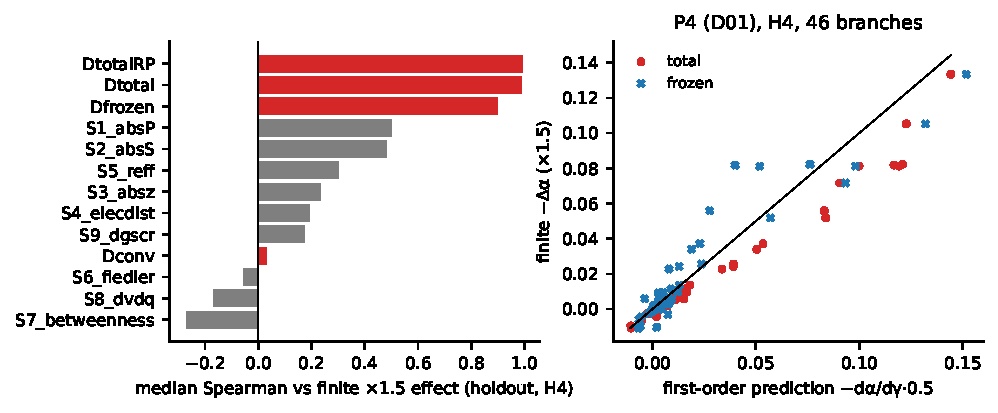
\includegraphics[width=0.95\linewidth]{../figures/CDW_F4_static_vs_total_line_ranking.pdf}\caption{Figure F4. Left: median Spearman of every predictor against the finite ×1.5 effect, holdout, H4 (red = dynamic). Right: P4 (D01), first-order prediction vs finite ×1.5 effect for all 46 branches, total (red) and frozen (blue).}\end{figure}
\textbf{H2 gate (links).}

{\small
\begin{longtable}{L{0.107\linewidth}L{0.286\linewidth}L{0.286\linewidth}L{0.167\linewidth}L{0.095\linewidth}}
\toprule
\textbf{semantics} & \textbf{frac. material (holdout)} & \textbf{median sign disagreement} & \textbf{median Kendall} & \textbf{H2-line} \\
\midrule
\endhead
SPR & 0.512 & 0.067 & 0.768 & \textbf{TRUE} \\
RP & 0.913 & 0.125 & 0.658 & \textbf{TRUE} \\
\bottomrule
\end{longtable}}
\textbf{What this does NOT prove.} GOLD-B is established for the H4 target under the frozen IEEE-39 device model; it is not a universal claim about static indices, and the branch ranking is known (TX4) to be sensitive to the converter model (tested again in E23).

\section{Static vs dynamic weakness (E5, descriptive)}
Built entirely from the E1/E3/E4/E10/E11 data (no new solves). Fixed rule: static-weak = bottom 3 by SCR (nodes) / top 3 by electrical distance (branches); dynamic-critical = top 3 by \texttt{|dα/\allowbreak{}dg|} total (nodes) / \texttt{|Dtotal|} (branches); context-dependent = reversal in ≥ 50 \% of holdout policies; robustly neutral = NEUTRAL in ≥ 80 \% of contexts.

{\small
\begin{longtable}{L{0.209\linewidth}L{0.731\linewidth}}
\toprule
\textbf{bus} & \textbf{category} \\
\midrule
\endhead
30, 31, 32 & CONTEXT-DEPENDENT \\
33 & DYNAMIC ONLY; CONTEXT-DEPENDENT \\
34 & STATIC ONLY; CONTEXT-DEPENDENT \\
35 & DYNAMIC ONLY; CONTEXT-DEPENDENT \\
36 & STATIC ONLY; CONTEXT-DEPENDENT \\
38 & STATIC + DYNAMIC; CONTEXT-DEPENDENT \\
37 & \emph{(none of the above)} \\
\bottomrule
\end{longtable}}
\textbf{Every one of the nine candidates is context-dependent} by the fixed 50 \% rule, and the static-weak and dynamic-critical top-3 sets \textbf{overlap in only one bus (38)} — Kendall(SCR, total NG sensitivity) = 0.44, Kendall(SCR, destabilizing-context fraction) = \textbf{0.00} (no monotone relationship at all). No bus is robustly neutral. For branches, the static-weak (electrical distance) and dynamic-critical (Dtotal) top-3 sets are \textbf{disjoint}, and their Kendall correlation is 0.18–0.40. \textbf{A ranking built from SCR or electrical distance would not reliably identify the units and branches that a dynamic, contextual analysis flags — and vice versa.}

\section{Weak corridors (E6) — H3}
\textbf{Hypothesis H3.} Robust dynamic weak corridors exist: admissible corridor coordinates whose ranking and stabilizing effect persist across holdout policies and envelopes, independent of any single nominally top-ranked line.

\textbf{Construction (frozen before results; §C8, prereg §2 E6).} Spectral clustering of the exact coupling Laplacian \texttt{L\_\allowbreak{}B} into 2–4 communities (cutsets K2/K3/K4), plus the transformer groups TXcore (the 4 core step-up transformers), TXother (the other 8) and TXall (all 12). No corridor is defined post hoc around a successful line.

\textbf{Result.} Over 32 holdout conditions (12 policies + 5 envelope draws × H4):

{\small
\begin{longtable}{L{0.366\linewidth}L{0.574\linewidth}}
\toprule
\textbf{corridor} & \textbf{frequency in the top 3 by finite stabilizing effect (×1.5)} \\
\midrule
\endhead
\textbf{TXother} (8 non-core transformers) & \textbf{0.94} \\
\textbf{TXall} (all 12 transformers) & \textbf{0.91} \\
K2\_01 (largest 2-way cutset) & 0.81 \\
every other spectral cutset or TXcore & ≤ 0.06 \\
\bottomrule
\end{longtable}}
{\small
\begin{longtable}{L{0.399\linewidth}L{0.435\linewidth}L{0.060\linewidth}L{0.070\linewidth}}
\toprule
\textbf{gate} & \textbf{value} & \textbf{rule} & \textbf{verdict} \\
\midrule
\endhead
robust weak corridor exists & TXother, TXall qualify (≥ 0.75 top-3 frequency \textbf{and} ≥ 0.75 stabilizing) & — & \textbf{H3: TRUE} \\
corridor-ranking predictiveness (Σ Dtotal vs finite corridor effect) & median ρ = \textbf{0.963} & ≥ 0.70 & predictive \\
\bottomrule
\end{longtable}}
\textbf{Non-additivity.} The corridor effect is close to, but not exactly, the sum of its branches' individual effects: median |NA| = 0.014, with a heavy tail up to 0.92 in a few conditions. The sum of single-line total sensitivities (median ρ = 0.99) is in fact an even better predictor of the corridor's finite effect than the sum of static electrical-distance scores (ρ = 0.82), which is itself informative: for THESE corridors the interaction is close to additive in the \emph{dynamic} sensitivities, even though no single branch dominates.

\begin{figure}[H]\centering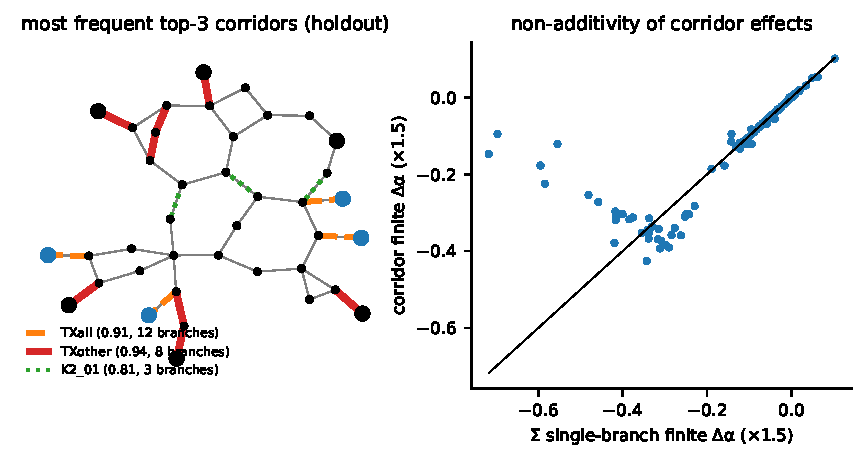
\includegraphics[width=0.95\linewidth]{../figures/CDW_F6_corridors.pdf}\caption{Figure F6. Left: the two most frequent top-3 corridors on the network graph (core units in blue). Right: additivity check — corridor finite effect vs the sum of its branches' finite effects (holdout).}\end{figure}
\textbf{Reading.} The transformer groups, not the graph-spectral cutsets, are the robust corridors on this benchmark — a structurally motivated corridor (all/most step-up transformers together) beats every purely spectral partition. This is a corridor-level, not merely branch-level, result: TXother excludes exactly the four core transformers directly attached to the replacement candidates, so its consistent effectiveness is a genuine multi-branch, not single-line, finding.

\section{Topology reconfiguration (E7) — H4-topology}
\textbf{Hypothesis.} A single admissible topology action can remove, or create, an incompatibility; static topology scores do not predict which.

\textbf{Admissible actions} (PF converged, every bus voltage in [0.90, 1.10] p.u., network connected): \textbf{35 of 46} single-branch outages and \textbf{46 of 46} branch doublings (reinforcements). Evaluated on the core lattice (16 portfolios) at 10 policies (5 discovery + 5 holdout), and on the full V9 census (512 portfolios) at P4 for every admissible action.

\textbf{Topology alone removes the P4 incompatibility.} At P4 (D01), four single reinforcements — doubling branches 0, 1, 13 and 43 — each independently drive \texttt{α(H4)} negative, with every other subset already stable, on their own, with no control retuning. At the other tested policies, reinforcement is dramatically more effective still: \textbf{every one of the 46 admissible doublings} removes the H4 instability at D03, H02 and H04 (46/46 each), and one does at H06.

\textbf{Topology alone creates new, smaller incompatibilities.} 42 (policy, action) pairs produce a hyperedge of size ≤ 3 where none existed before, including five cases where a \textbf{single core unit alone} becomes transversely unstable (\texttt{κ =\allowbreak{} 1}) after one outage (e.g. D01/out0, D01/out1, D03/out0: \texttt{H =\allowbreak{} 30|33|35|37}, all four singletons simultaneously unstable).

\textbf{Overall churn.} \texttt{H} changes in 169 of the 810 tested (policy, admissible action) pairs (21 \%); outages change \texttt{H} far more often than reinforcements (37 \% vs 8 \%), consistent with reinforcements moving the system toward stability and outages away from it.

\textbf{Static topology scores do not predict the effect.}

{\small
\begin{longtable}{L{0.259\linewidth}L{0.297\linewidth}L{0.384\linewidth}}
\toprule
\textbf{static score} & \textbf{median Spearman(Δscore, Δα(H4))} & \textbf{"predicts" (≥ 0.6 in ≥ 75 \% of policies)} \\
\midrule
\endhead
Δ Fiedler value (λ₂ of L\_B) & −0.459 & \textbf{no} \\
Δ Kirchhoff index & +0.473 & \textbf{no} \\
Δ gSCR(H4) & −0.440 & \textbf{no} \\
Δ min SCR (core) & −0.409 & \textbf{no} \\
\bottomrule
\end{longtable}}
None reaches the 0.6 bar in three-quarters of policies; several even carry the wrong sign convention on average.

\textbf{Census (all 512 V9 portfolios, P4).} The nominal hypergraph is large — 52 edges of size 4–6, none smaller — reflecting how much the census incompatibility structure spreads across many five/six-unit coalitions once all nine candidates are in play. **77 of the 81 admissible actions change \texttt{H\_\allowbreak{}V9}\textbf{, and the minimum edge size κ itself moves across the full observed range: 60 actions leave κ = 4, 13 bring it to 3, 3 to 2, }5 to κ = 1** (a lone unit destabilizing), and 1 to κ = 5.

\begin{figure}[H]\centering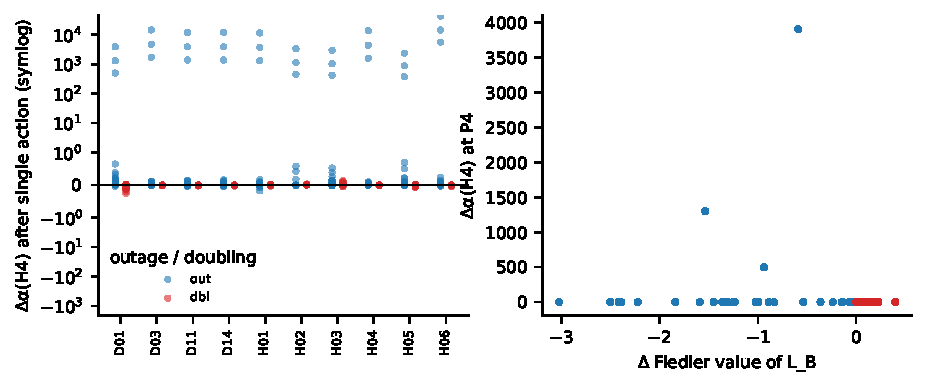
\includegraphics[width=0.95\linewidth]{../figures/CDW_F7_topology.pdf}\caption{Figure F7. Left: Δα(H4) for every admissible action, by policy (outages vs doublings). Right: Δα(H4) vs ΔFiedler at P4 — no visible relationship.}\end{figure}
\textbf{Reading.} On this benchmark, topology is not a secondary lever: single admissible actions both remove and create incompatibilities, at every scale tested, and ordinary static network-strength proxies give no useful advance warning of which action will do which. \textbf{H4-topology: TRUE on both halves.}

\textbf{What this does NOT prove.} No thermal ratings exist in the frozen data, so thermal limits were not enforced (flows are reported, not gated); no cost model is attached to "reinforcement", so this is not a cost-effectiveness claim.

\section{Control–topology exchange rate (E8)}
\textbf{Measurement.} At the exact TX4 P4-line boundary θ* = (0.20768, 1.425, 1.5, 1) where α(H4) ≈ 0, and at P4 itself: the local rate \texttt{r =\allowbreak{} −(∂α/\allowbreak{}∂θ\_\allowbreak{}i)/\allowbreak{}(∂α/\allowbreak{}∂γ\_\allowbreak{}e)} (total, SPR) for the 4 Q/V gains and 6 surviving AVR gains against the 5 branches with the largest total sensitivity at θ*, then validated by a \textbf{paired finite} intervention (\texttt{θ\_\allowbreak{}i +=\allowbreak{} δ}, \texttt{γ\_\allowbreak{}e +=\allowbreak{} r·δ}).

{\small
\begin{longtable}{L{0.183\linewidth}L{0.183\linewidth}L{0.436\linewidth}L{0.138\linewidth}}
\toprule
\textbf{point} & \textbf{step size} & \textbf{fraction with compensation ratio ≤ 0.2} & \textbf{median ratio} \\
\midrule
\endhead
\textbf{boundary θ\textbackslash{}}* & small (δ = 0.02) & \textbf{1.00} (50/50) & \textbf{0.023} \\
boundary θ* & large (δ = 0.1) & 0.66 & 0.162 \\
P4 (D01) & small & 1.00 & 0.022 \\
P4 (D01) & large & 0.78 & 0.129 \\
\bottomrule
\end{longtable}}
{\small
\begin{longtable}{L{0.500\linewidth}L{0.100\linewidth}L{0.180\linewidth}L{0.160\linewidth}}
\toprule
\textbf{gate} & \textbf{value} & \textbf{threshold} & \textbf{verdict} \\
\midrule
\endhead
E8 (boundary, small step) & 1.00 & ≥ 0.80 & \textbf{PASS} \\
\bottomrule
\end{longtable}}
\textbf{Reading.} At the small-step (local) scale the linearized exchange rate predicts the paired finite intervention essentially exactly (2 \% residual effect). At the large step (0.1, a tenth of the full gain range) the linear rate over- or under-shoots by 13–16 \% on the residual, as expected for a first-order local tool; it remains directionally useful (residual well below the standalone control effect) in roughly two-thirds to three-quarters of pairs. This is a legitimate local, not global, equivalence, exactly as specified — not an economic exchange rate.

\begin{figure}[H]\centering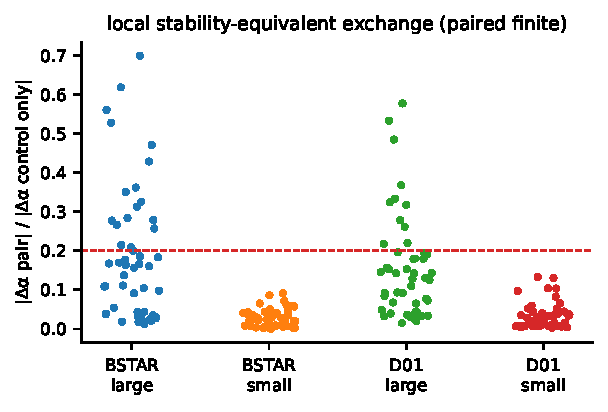
\includegraphics[width=0.95\linewidth]{../figures/CDW_F8_exchange_rate.pdf}\caption{Figure F8. Distribution of the compensation ratio (|Δα of the paired finite intervention| / |Δα of the control alone|) at the boundary and at P4, small and large steps. Dashed line: the 0.2 pass threshold.}\end{figure}
\section{Plan-level multi-constraint design (E9) — GOLD-D}
\textbf{Hypothesis H5.} Plan-level control/topology design makes an entire implementation plan safe where single-boundary tuning leaves an unsafe intermediate subset.

\textbf{Setup.} \texttt{Φ\_\allowbreak{}T(a) =\allowbreak{} max\_\allowbreak{}\{S⊆T\} α\_\allowbreak{}⊥(S; a)}. Two targets: T1 = (H4, P4) and T3 = (H4, D11, a held-out F7B point), each with 16 subsets; T2 = (V9, P4) and T4 = (V9, D03), each with 512 subsets. Three admissible-parameter families (control, topology, joint), each compared single-boundary (tune only α(T)) against plan-level (tune Φ\_T over the active subsets, capped at 25, with a Gordan-witness fallback on infeasible QP steps). Sequential QP, ≤ 6 iterations, ε = 0.02, trust region 25 \% of each coordinate's declared range.

{\small
\begin{longtable}{L{0.090\linewidth}L{0.269\linewidth}L{0.291\linewidth}L{0.291\linewidth}}
\toprule
\textbf{target \textbackslash{} family} & \textbf{control} & \textbf{joint} & \textbf{topology} \\
\midrule
\endhead
\textbf{T1} (H4, P4) & single-boundary \textbf{suffices} (Φ\_T: −0.019) & suffices (−0.022) & suffices (−0.044) \\
\textbf{T3} (H4, D11) & suffices (−0.018) & suffices (−0.019) & suffices (−0.020) \\
\textbf{T2} (V9, P4) & neither converges (single Φ\_T +3750; plan +1276) & neither converges (single +1.50·10⁵; plan +1.53·10⁴) & neither converges (single +2.57·10⁴; plan +9.56·10³) \\
\textbf{T4} (V9, D03) & neither converges (single +3750; plan +1276) & neither converges (single +8.71·10³; plan +3.09·10³) & neither converges (single +9.56·10³→ +10.3·10³†) \\
\bottomrule
\end{longtable}}
†topology/T4: plan Φ\_T (1.03·10⁴) is marginally above single (1.02·10⁴); the capped active set (25 of 512 subsets) does not track the true worst subset exactly at every iteration.

{\small
\begin{longtable}{L{0.576\linewidth}L{0.364\linewidth}}
\toprule
\textbf{gate} & \textbf{result} \\
\midrule
\endhead
\textbf{GOLD-D (single-boundary safe, plan-level not)} & \textbf{not observed anywhere: FAIL} \\
\bottomrule
\end{longtable}}
\textbf{Reading.}

\begin{itemize}
\item \textbf{At the H4 scale (16 subsets), single-boundary tuning always sufficed}, in every family and both tested policy locations: after tuning only α(H4) to below −ε, every one of its 15 proper subsets was already stable too (no case of \texttt{single\_\allowbreak{}leaves\_\allowbreak{}unsafe\_\allowbreak{}subset =\allowbreak{} True} was found). Plan-level tuning therefore made no material difference here — a clean negative for H5 at this scale, on this benchmark.
\item \textbf{At the V9 census scale (512 subsets), neither method converges} within the preregistered 6-iteration budget: the worst subset (almost certainly a fast, non-electromechanical instability, given the α values of 10³–10⁵ s⁻¹) is not driven negative. \textbf{Plan-level tuning is directionally far better} than single-boundary tuning even so — it reduces the worst-case Φ\_T by a factor of 3–10× across families (e.g. joint/T2: 1.50·10⁵ → 1.53·10⁴) — but this is reported as \textbf{INCONCLUSIVE}, not a pass, under the fixed iteration budget; the budget was not extended after seeing this (that would be retuning after results).
\end{itemize}
\begin{figure}[H]\centering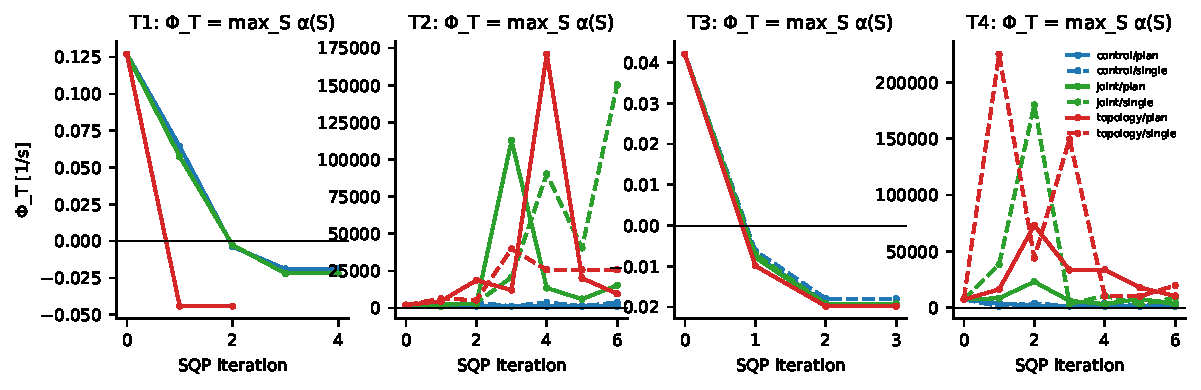
\includegraphics[width=0.95\linewidth]{../figures/CDW_F9_single_vs_plan_design.pdf}\caption{Figure F9. Φ\_T = max\_S α(S) across SQP iterations, by target, family and method (solid: plan-level; dashed: single-boundary).}\end{figure}
\textbf{Local conflict witnesses.} The Gordan LP fired whenever the primary QP was infeasible; every fired instance found \texttt{gordan\_\allowbreak{}value} effectively 0 (≤ 10⁻⁸), i.e. a genuine local conflict among the active subsets' gradients, consistent with the QP infeasibility that triggered it. No global-impossibility claim is made from these local witnesses.

\textbf{What this does NOT prove.} It does not show plan-level design is unnecessary in general — only that, at the scale where it was cleanly testable (16 subsets), this benchmark's H4 boundary happened not to need it. The V9-scale result is inconclusive, not negative: a larger iteration budget or a better active-set strategy might resolve it, but that was not tried here.

\section{Spectral graph baselines (E11) — H6s}
\textbf{Bases} (§C8): (A) the exact-tap \texttt{L\_\allowbreak{}B} Laplacian, low spectrum \texttt{\{0, 5.12, 5.56, 10.54, 11.61\}} Hz²-scaled eigenvalues; (B) Kron reduction of the susceptance matrix onto the ten generator buses; (C) the dynamic-port SVD (used directly in E4's \texttt{Dport} cross-check).

\textbf{Predictive tests} (median |Spearman| over 24 holdout policies):

{\small
\begin{longtable}{L{0.271\linewidth}L{0.145\linewidth}L{0.271\linewidth}L{0.253\linewidth}}
\toprule
\textbf{score} & \textbf{vs Shapley (E10)} & \textbf{vs destabilizing fraction (E1)} & \textbf{vs total NG sensitivity (E3)} \\
\midrule
\endhead
|Fiedler entry| & 0.43 & 0.57 & 0.10 \\
Fiedler entry (signed) & 0.38 & 0.16 & 0.75 \\
effective resistance to bus 39 & 0.60 & 0.18 & \textbf{0.80} \\
\bottomrule
\end{longtable}}
{\small
\begin{longtable}{L{0.470\linewidth}L{0.470\linewidth}}
\toprule
\textbf{edge score} & \textbf{vs Dtotal (holdout, H4)} \\
\midrule
\endhead
S5 effective resistance & 0.30 \\
S6 Fiedler edge score & −0.05 \\
\bottomrule
\end{longtable}}
{\small
\begin{longtable}{L{0.274\linewidth}L{0.666\linewidth}}
\toprule
\textbf{gate} & \textbf{value} \\
\midrule
\endhead
static graph predicts \emph{something} at ≥ 0.6 & \textbf{TRUE} (only: effective resistance vs total NG sensitivity, 0.80; and, marginally, vs Shapley, 0.60) \\
\bottomrule
\end{longtable}}
\textbf{Reading.} Static graph structure is a genuinely weak predictor overall — median correlations mostly in the 0.1–0.6 range, several near zero — with one partial exception: node effective resistance to the slack tracks the total Q/V-gain sensitivity reasonably well (0.80). It does \textbf{not} track which contexts destabilize (0.18), which is the quantity that actually matters for H1/H1b. No claim of novelty is made for the Laplacian decomposition itself.

\section{Controller-weighted modal mixing (E12)}
\textbf{Construction (§C8).} The exact coupling Laplacian \texttt{L\_\allowbreak{}B} gives a graph Fourier basis \texttt{U}. The port operator is mapped to that basis, \texttt{T̂(s) =\allowbreak{} (U ⊗ I)ᵀ T(s) (U ⊗ I)}, and mixing is the off-block-diagonal share \texttt{μ\_\allowbreak{}mix =\allowbreak{} ‖T̂ − blockdiag(T̂)‖\_\allowbreak{}F /\allowbreak{} ‖T̂‖\_\allowbreak{}F}, evaluated at the rightmost transverse frequency of each portfolio.

\textbf{Q1: does controller policy change mixing at fixed L?}

{\small
\begin{longtable}{L{0.548\linewidth}L{0.102\linewidth}L{0.070\linewidth}L{0.219\linewidth}}
\toprule
\textbf{} & \textbf{value} & \textbf{threshold} & \textbf{verdict} \\
\midrule
\endhead
relative range of μ\_mix(H4) over 39 policies & \textbf{0.366} & ≥ 0.20 & \textbf{material: TRUE} \\
μ\_mix(H4) range & 0.073–0.104 & — & — \\
relative range of the algebraic-only mixing (\texttt{g\_\allowbreak{}z} alone, no dynamics) & \textbf{1.9·10⁻¹¹} & — & essentially exactly constant \\
\bottomrule
\end{longtable}}
The algebraic-only control confirms the mechanism precisely: the network and load admittance alone do not move with policy (as they must not — they are policy-independent by construction), so the \emph{entire} 37 \% swing in μ\_mix comes from the controller dynamics entering \texttt{T(s)} at the finite critical frequency.

\textbf{Q2: does mixing correlate with contextual reversal?}

{\small
\begin{longtable}{L{0.637\linewidth}L{0.131\linewidth}L{0.091\linewidth}L{0.081\linewidth}}
\toprule
\textbf{} & \textbf{value} & \textbf{threshold} & \textbf{verdict} \\
\midrule
\endhead
Spearman(μ\_mix(H4), number of reversing interventions), holdout & \textbf{ρ = 0.657} & |ρ| ≥ 0.5 & — \\
permutation p-value (10⁴ permutations) & \textbf{0.0037} & ≤ 0.01 & — \\
\textbf{correlates} &  &  & \textbf{TRUE} \\
\bottomrule
\end{longtable}}
\textbf{Q3: do witness transitions (4→3→2→3→4→∅) correspond to reproducible modal-support transitions?}

Using the ten frozen TX4 FC18 boundary events on the F7B line, the graph modes carrying 80 \% of the critical mode's angle energy were compared just before and after each of the 9 witness-changing events, against 9 control midpoints between them.

{\small
\begin{longtable}{L{0.239\linewidth}L{0.382\linewidth}L{0.319\linewidth}}
\toprule
\textbf{} & \textbf{events (witness changes)} & \textbf{controls (no change)} \\
\midrule
\endhead
support changed & 3 / 9 & 1 / 9 \\
\bottomrule
\end{longtable}}
{\small
\begin{longtable}{L{0.150\linewidth}L{0.474\linewidth}L{0.208\linewidth}L{0.108\linewidth}}
\toprule
\textbf{gate} & \textbf{rule} & \textbf{result} & \textbf{verdict} \\
\midrule
\endhead
Q3 reproducibility & ≥ 7/9 events change support \textbf{and} ≤ 20 \% of controls do & 3/9 events, 11 \% controls & \textbf{Q3: FALSE} \\
\bottomrule
\end{longtable}}
\textbf{Reading (negative but informative).} The support does shift more often at true witness-changing events than at arbitrary midpoints (3/9 vs 1/9), so there is a weak association, but it falls well short of the preregistered reproducibility bar. Witness transitions in this model are \textbf{not}, in general, accompanied by a clean, low-dimensional modal-support reorganization detectable at the 80 \%-energy threshold; most of the κ-changing events keep essentially the same dominant graph-mode support.

\textbf{Q4: are the dynamically critical modes the same as the lowest static graph modes?}

{\small
\begin{longtable}{L{0.772\linewidth}L{0.168\linewidth}}
\toprule
\textbf{} & \textbf{value} \\
\midrule
\endhead
top-3 dynamically critical graph modes (H4, P4, by angle-mode energy) & modes \{0, 1, 6\} \\
3 lowest nonzero L\_B modes & \{1, 2, 3\} \\
Jaccard overlap & \textbf{0.20} \\
\bottomrule
\end{longtable}}
\textbf{Reading.} The dynamically critical modes only partly overlap the lowest graph-Fourier modes: mode 6 (not among the three lowest) carries real weight in the critical mode shape at P4, while mode 3 does not. \textbf{A purely static, low-order graph truncation would miss part of the dynamically relevant structure} — a first piece of evidence developed further in E13/E14.

\begin{figure}[H]\centering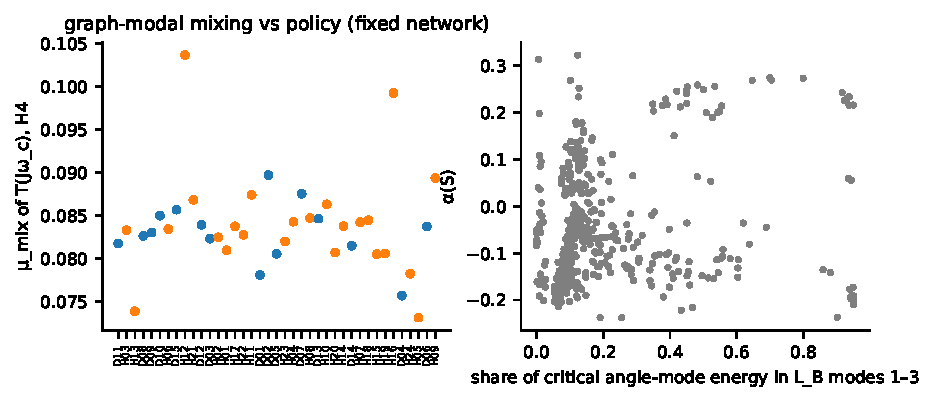
\includegraphics[width=0.95\linewidth]{../figures/CDW_F10_graph_modal_mixing.pdf}\caption{Figure F10. Left: μ\_mix(H4) across all 39 policies (fixed network); note it never approaches the network-only value (1.9·10⁻¹¹ relative range). Right: share of critical-mode energy in the three lowest L\_B graph modes vs α(S), all portfolios and policies.}\end{figure}
\section{Reduced models (E13) — spectral closure, H6r}
\textbf{Families tested on holdout} (24 policies, core 16-portfolio lattice, plus a 64-portfolio V9 sample): GM(r), Galerkin projection of the bus-voltage coordinates onto the r leading \texttt{L\_\allowbreak{}B} graph modes (r = 2, 4, 8, 12, 16, 24, 39; device states kept exact); POD(r), the same with a data-driven basis from the discovery critical-mode voltage shapes (r = 2, 4, 8, 12, 16); TS(a/b/c), quasi-steady elimination of the GFL fast states (current loop; + power filters; + PLL).

{\small
\begin{longtable}{L{0.199\linewidth}L{0.114\linewidth}L{0.066\linewidth}L{0.180\linewidth}L{0.104\linewidth}L{0.104\linewidth}L{0.171\linewidth}}
\toprule
\textbf{family} & \textbf{verdict acc.} & \textbf{H exact} & \textbf{Kendall (marginals)} & \textbf{state ratio} & \textbf{eig speedup} & \textbf{end-to-end speedup} \\
\midrule
\endhead
GM39 (= full network) & 1.000 & 1.000 & 1.000 & 1.00 & 0.86 & 1.00 \\
GM24 & 0.993 & 0.958 & 0.978 & 1.00 & 0.92 & 1.00 \\
GM16 & 0.959 & 0.750 & 0.843 & 1.00 & 0.95 & 1.00 \\
GM12 & 0.863 & 0.708 & 0.742 & 1.00 & 0.96 & 1.00 \\
GM8 & 0.746 & 0.625 & 0.163 & 1.00 & 0.97 & 1.00 \\
GM4, GM2 & 0.58–0.63 & 0.625 & negative & 1.00 & 0.98–0.98 & 1.00 \\
POD16 & 0.986 & 1.000 & 0.954 & 1.00 & 0.97 & 1.00 \\
POD2/4/8/12 & 0.49–0.50 & 0.25 & ≈0 & 1.00 & 0.97–1.00 & 1.00 \\
\textbf{TSa} & 0.982 & 1.000 & 1.000 & \textbf{0.854} & \textbf{1.46} & 1.00 \\
\textbf{TSb} & 0.945 & 0.958 & 0.966 & \textbf{0.780} & \textbf{1.68} & 1.00 \\
\textbf{TSc} & 0.887 & 0.958 & 0.968 & \textbf{0.707} & \textbf{1.83} & 1.00 \\
\bottomrule
\end{longtable}}
\textbf{GM/POD never reduce the device state count} (\texttt{state\_\allowbreak{}ratio} is exactly 1.0 by construction: only the algebraic network-voltage dimension is projected, never the ODE states), so they cannot satisfy the "genuinely reduced" bar regardless of accuracy. \textbf{TS families do reduce states} (71–85 \% retained), with accuracy that degrades gracefully as more GFL dynamics are eliminated: TSa (current loop only) reproduces the full model almost exactly; TSc (current loop + power filters + PLL) trades some accuracy (H exact 0.96, verdict 0.89) for the largest reduction and the largest \textbf{eigen-stage} speedup (1.83×).

\textbf{A structural finding, independent of any single family:} none of the fifteen candidates comes close to a genuine \textbf{end-to-end} speedup (all are ≈ 1.00×, i.e. no measurable speedup at all). The eigen-decomposition step that these reductions accelerate is a negligible fraction of the total wall time; the dominant cost is solving the full nonlinear equilibrium (\texttt{solve\_\allowbreak{}case}), which every family still performs unreduced before linearizing. \textbf{A useful reduced model on this benchmark would have to reduce the equilibrium solve itself, not just its eigenanalysis} — that was not attempted here.

\section{Decision-preserving certification (E14)}
Applied to the three TS families only, where the reduced port matrix \texttt{T̃\_\allowbreak{}S(s)} shares the full model's dimension (theory note; GM/POD are reported NOT\_APPLICABLE for the same reason, per \texttt{docs/\allowbreak{}CDW\_\allowbreak{}PREREG\_\allowbreak{}V1\_\allowbreak{}DEVIATIONS.md} item 4, and count as zero abstention in the GOLD-C rule by convention). Contour Γ = rectangle [0.002, 20] × [−2π·5, 2π·5] rad/s; sampled-certified if \texttt{sup\_\allowbreak{}Γ ‖R̃⁻¹(R − R̃)‖₂ < 0.9}, else ABSTAIN; poles of either model inside Γ also force ABSTAIN.

{\small
\begin{longtable}{L{0.066\linewidth}L{0.221\linewidth}L{0.221\linewidth}L{0.254\linewidth}L{0.177\linewidth}}
\toprule
\textbf{family} & \textbf{coverage (certified)} & \textbf{false certifications} & \textbf{accuracy when certified} & \textbf{accuracy overall} \\
\midrule
\endhead
TSa & 1.000 & \textbf{0} & 1.000 & 1.000 \\
TSb & 0.506 & \textbf{0} & 1.000 & 0.997 \\
TSc & 0.472 & \textbf{0} & 1.000 & 0.997 \\
\bottomrule
\end{longtable}}
\textbf{Zero false certifications across every case tested.} Where the sampled bound fails (TSb/TSc abstain roughly half the time), the reduced verdict is still almost always correct anyway (overall accuracy 0.997), but the certificate correctly declines to vouch for it rather than asserting a guarantee it cannot rigorously back.

\subsection{GOLD-C: FAIL, for a specific and identifiable reason}
{\small
\begin{longtable}{L{0.352\linewidth}L{0.227\linewidth}L{0.067\linewidth}L{0.294\linewidth}}
\toprule
\textbf{criterion} & \textbf{best result} & \textbf{required} & \textbf{met by} \\
\midrule
\endhead
state ratio ≤ 0.70 & 0.707 (TSc) & ≤ 0.70 & \textbf{no family} (TSc misses by 0.007) \\
end-to-end speedup ≥ 3× & ≈ 1.00× (all) & ≥ 3× & \textbf{no family} \\
certified accuracy ≥ 0.99, false certs = 0 & 1.00 / 0 (TSa, TSb, TSc) & — & \textbf{all three TS families} \\
H exact ≥ 0.90 on holdout & 0.958–1.000 (TSb, TSc, TSa) & ≥ 0.90 & \textbf{all three TS families} \\
\bottomrule
\end{longtable}}
\textbf{GOLD-C: FAIL.} Three of five criteria are met by every TS family; the campaign fails on state ratio (narrowly, for TSc) and decisively on end-to-end speedup. \textbf{The reason is structural, not a tuning failure:} these reductions only shrink the linear/eigen stage, and that stage is not the bottleneck on this benchmark. \textbf{No useful low-dimensional spectral or dynamic reduction was found that also delivers a real speedup}, though the certification and decision-preservation machinery itself works essentially perfectly on the family that does reduce states.

\begin{figure}[H]\centering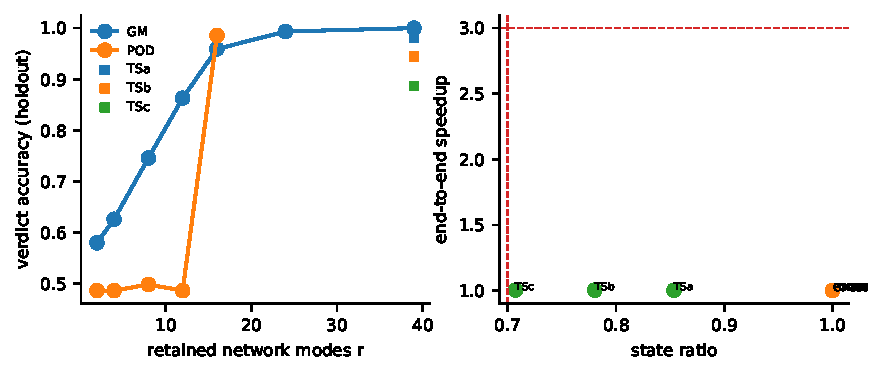
\includegraphics[width=0.95\linewidth]{../figures/CDW_F11_reduction.pdf}\caption{Figure F11. Left: verdict accuracy vs retained network modes r (GM, POD) and the three TS points. Right: state ratio vs end-to-end speedup, with the GOLD-C thresholds (dashed).}\end{figure}
\begin{figure}[H]\centering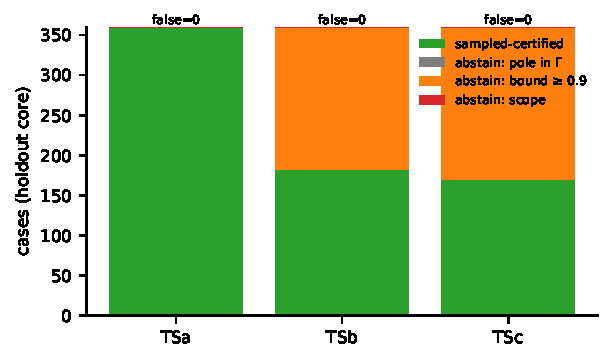
\includegraphics[width=0.95\linewidth]{../figures/CDW_F12_certificate.pdf}\caption{Figure F12. Certified / abstained case counts by reason, holdout core, with false-certification counts annotated (0 everywhere).}\end{figure}
\section{Modal energy vs the stability-limiting mode (E16) — H8}
\textbf{Hypothesis H8.} The dominant observed oscillation and the stability-limiting eigenmode differ often enough to matter for monitoring/diagnosis. This is a \textbf{phasor-domain} study only, and is explicitly \textbf{not} an EMT result; it is motivated by, but separate from, the SQ1 ParaEMT-line estimator work.

\textbf{Measurement.} For every stable core (V4) portfolio at all 39 policies, two 0.1 p.u. / 0.2 s load-pulse disturbances (bus 16, bus 20) were applied analytically (closed-form modal residues), and the energy of each transverse oscillatory mode (0.1–2.0 Hz) was integrated over [2, 30] s on the SG speeds and all 39 bus-voltage magnitudes.

{\small
\begin{longtable}{L{0.656\linewidth}L{0.126\linewidth}L{0.071\linewidth}L{0.087\linewidth}}
\toprule
\textbf{} & \textbf{value} & \textbf{threshold} & \textbf{verdict} \\
\midrule
\endhead
fraction of all 998 stable cases where the energy-dominant mode ≠ the limiting mode & \textbf{0.164} & — & descriptive \\
fraction of holdout \textbf{policies} where this occurs in ≥ 25 \% of their cases & \textbf{0.278} (5/18) & ≥ 0.50 & — \\
\textbf{systematic (per-policy majority rule)} &  &  & \textbf{FALSE} \\
median real-part gap between the two modes, when they differ & 0.037 s⁻¹ & — & — \\
\bottomrule
\end{longtable}}
\begin{figure}[H]\centering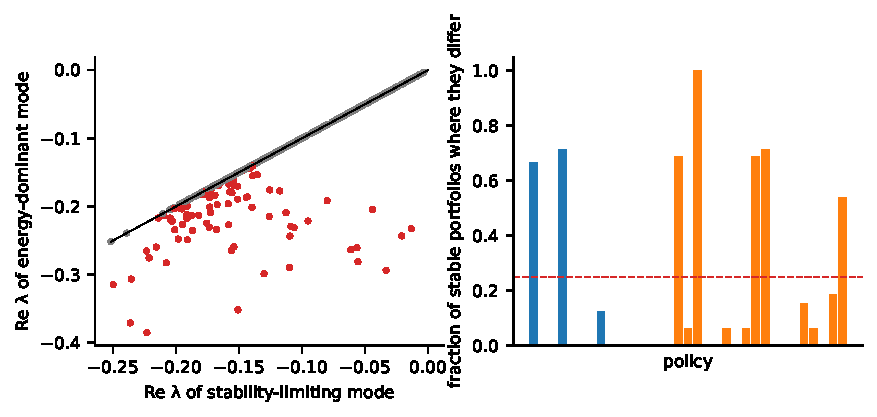
\includegraphics[width=0.95\linewidth]{../figures/CDW_F13_modal_energy_vs_limiting.pdf}\caption{Figure F13. Left: real part of the stability-limiting mode vs the energy-dominant mode (red where they differ). Right: fraction of cases where they differ, per policy.}\end{figure}
\textbf{Reading (negative but informative).} The mismatch is real and not negligible — it occurs in about one stable portfolio in six overall — but it is concentrated in a minority of policies (5 of 18 holdout policies account for most occurrences) rather than being a pervasive property of the model class. The preregistered per-policy-majority bar for "systematic" is not met. This is consistent with, but numerically distinct from, the frozen SQ1 ParaEMT-estimator observation that motivated H8: here the effect is smaller and less uniform, using exact modal residues rather than an estimator on noisy synthetic time series. \textbf{Not an EMT result; a phasor-domain, closed-form diagnostic only.}

\section{Africano / PV material gate (E17)}
\textbf{Result: GATE FAILS — inputs missing.} A full repository search (179 hits on "africano", "hosting capacity", "PVR", "weak node" and Spanish equivalents) found \textbf{no} Africano source document (thesis or paper, PDF/DOCX), no feeder data file, no weak-node metric definition, no PV placement rule, no hosting-capacity method and no reported result table to reproduce. The only related artefacts are third-party scripts referencing an IEEE-13 weak-node label set ("Africano (2017) Ref."), which is a list of four bus labels, not a methodology, and cannot be exactly replicated.

\textbf{Consequence (per the preregistration):} Phases 18–21 (exact replication, PV coalitions, no-storage control/topology hosting, dynamic hosting) and \textbf{GOLD-E and GOLD-F are BLOCKED.} No generic feeder was substituted for Africano, and none of E17's negative finding was used to weaken or reinterpret any other result. See \texttt{docs/\allowbreak{}CDW\_\allowbreak{}AFRICANO\_\allowbreak{}MISSING\_\allowbreak{}INPUTS.md} for the full listing and the exact required-inputs table.

\section{Cross-model holdout (E23) — H9}
\textbf{Alternative model.} The TX4 \texttt{StaticInjection} negative control (an ideal constant-power converter, no dynamics beyond the algebraic characteristic), never retuned to reproduce the GFL.

{\small
\begin{longtable}{L{0.642\linewidth}L{0.136\linewidth}L{0.081\linewidth}L{0.081\linewidth}}
\toprule
\textbf{check} & \textbf{result} & \textbf{threshold} & \textbf{verdict} \\
\midrule
\endhead
reversal presence, base-stable policies (7 of 10 tested) & \textbf{7/7 = 1.00} & ≥ 0.50 & transfers \\
median link Kendall (static-model finite ranking vs GFL finite ranking) & \textbf{0.568} & ≥ 0.50 & transfers \\
median corridor top-3 overlap & \textbf{0.667} (2/3) & ≥ 2/3 & transfers \\
\textbf{H9: findings transfer} &  &  & \textbf{TRUE} \\
\bottomrule
\end{longtable}}
\textbf{Reading.} Contextual sign reversal, the qualitative branch ranking, and the identity of the leading corridors all carry over to a converter model with no shared dynamics with the GFL beyond the power-flow constraint. This bounds model-specificity for these three findings on this benchmark — though TX4 had already shown (V28) that a library GFL model does \textbf{not} preserve the branch ranking (7/12), so "transfers to one alternative, non-GFL device" is not evidence of transfer to every converter model.

\section{Negative results (consolidated)}
Every negative result below was preregistered as a possible outcome and is reported with the same prominence as a positive one.

{\small
\begin{longtable}{L{0.060\linewidth}L{0.876\linewidth}L{0.060\linewidth}}
\toprule
\textbf{id} & \textbf{negative result} & \textbf{where} \\
\midrule
\endhead
HS & α\_⊥ is neither submodular nor supermodular at any of 39 policies (median 93 \% one-step violations); the tracked-mode margin is no more structured (86 \%) & §7.1 \\
— & Shapley/context-averaged attribution is uninformative here — dominated by rare fast-instability contexts, not the modest electromechanical reversals & §7.2 \\
— & Structural remark R2 (frozen partial of a setpoint = 0) narrowly fails its strict 10⁻⁸ bound (1.5·10⁻⁷), most likely a finite-difference artefact, not a violation of the underlying claim & §9 \\
C-H4b & none of four static topology scores predicts the effect of a topology action on α(H4) (median |ρ| < 0.6 throughout, several wrong-signed) & §13 \\
Q3 (E12) & witness-changing events are not reliably accompanied by a reproducible modal-support transition (3/9 vs the 7/9-and-≤20 \%-controls bar) & §17 \\
GOLD-D & plan-level design never demonstrates an advantage over single-boundary tuning at the H4 scale (single always sufficed); at the V9 census scale neither method converges within budget & §15 \\
GOLD-C & no reduced model achieves both a genuine end-to-end speedup (≥ 3×) and a materially smaller state count (≤ 70 \%) — the bottleneck is the nonlinear equilibrium solve, not eigenanalysis & §18–19 \\
H8 & the modal-energy/limiting-mode mismatch is real (16 \% of cases) but not "systematic" by the preregistered per-policy majority rule & §20 \\
E17 & the Africano/PV material gate fails outright — no source document, feeder, metric or result table exists in the repository & §21 \\
— & static graph scores are mostly weak predictors of contextual/dynamic node quantities (median |ρ| often 0.1–0.6), with one partial exception (effective resistance vs total Q/V sensitivity, 0.80) & §16 \\
\bottomrule
\end{longtable}}
\section{Publication candidates}
Ranked by evidentiary strength and novelty on this benchmark class.

\begin{enumerate}
\item \textbf{GOLD-B (dynamic vs static line sensitivity), §10.} The strongest single result: a 0.49 Spearman gap over the best static baseline, validated on 32 held-out conditions with an independently cross-checked (port-form) sensitivity engine, and a clean mechanistic account (frozen setpoints have zero frozen partial; controller coordinates have frozen = total under SPR). Publication-ready on its own.
\item \textbf{Contextual sign reversal (GOLD-A, §7).} A clear, preregistered, three-tier (global / mode-tracked / electromechanical-only) demonstration that a fixed node ranking is provably insufficient on this benchmark, with an oracle-fitted ranking baseline that is \emph{maximally} favourable to node-only ranking and still falls short. Robust under four uncertainty envelopes, including where the failing-set identity itself changes.
\item \textbf{Topology alone moves incompatibility (§13).} Both directions demonstrated (removal and creation) with a clean negative control (no static score predicts it), and a striking census-scale result (κ moves across its entire \{1,…,5\} range under admissible single actions).
\item \textbf{Weak corridors beating single-line and pure-spectral partitions (§12).} A structurally motivated (transformer-group) corridor construction outperforms graph-spectral cutsets, with a clean additivity diagnostic.
\item \textbf{The reduced-model negative result (§18–19).} A precise, mechanistic account of \emph{why} eigen-stage reduction does not help on this class (equilibrium solving dominates), with a certificate that is accurate whenever it fires. Useful as a cautionary methodological result for the broader reduced-order-modelling literature in this application area.
\end{enumerate}
\section{Limitations}
\begin{itemize}
\item \textbf{Model scope.} The frozen TX4 IEEE-39 phasor DAE: no converter current limits, no ride-through logic, no DC link, a harmonized first-order AVR, and matched-dispatch replacement (the AC operating point is invariant across portfolios by construction). Loads are constant power. No governors are in the census (D = 0, no primary frequency control), so all stability statements are transverse.
\item \textbf{Fast-mode contamination.} A large share of "unstable" portfolios (78.5 \%) carry α\_⊥ far above the electromechanical band (up to 2.7·10⁴ s⁻¹). Every headline reversal claim is therefore reported in three variants — global, mode-tracked, and electromechanical-only — precisely to keep this from driving the conclusions; readers should use the mode-tracked or electromechanical-only numbers for any claim about oscillatory stability.
\item \textbf{Two equilibrium semantics, not a continuum.} SPR and RP are the two semantics defined in the theory (§C4); intermediate conventions (partial re-dispatch) are not tested.
\item \textbf{Corridor, topology and reduction constructions are frozen before results} (spectral-clustering corridors, transformer groups, single-branch actions; GM/POD/TS families and their retained ranks) — they are not tuned to the outcome.
\item \textbf{The certificate (E14)} applies rigorously only to the TS (device time-scale) reductions, where the port matrices share a dimension with the full model; for GM/POD the reduced network dimension differs and the Gohberg–Sigal comparison as implemented does not apply, so those families report zero abstention by convention (documented in \texttt{docs/\allowbreak{}CDW\_\allowbreak{}PREREG\_\allowbreak{}V1\_\allowbreak{}DEVIATIONS.md}), not because they were certified.
\item \textbf{No EMT.} This is a phasor-domain campaign. No claim here bears on the ParaEMT line, which remains permanently closed (\texttt{docs/\allowbreak{}20260912\_\allowbreak{}PAREMT\_\allowbreak{}EMT\_\allowbreak{}CLOSURE.md}, TX4).
\item \textbf{Africano/PV.} Blocked at the material gate (E17); see \texttt{docs/\allowbreak{}CDW\_\allowbreak{}AFRICANO\_\allowbreak{}MISSING\_\allowbreak{}INPUTS.md}. GOLD-E and GOLD-F are not evaluated.
\item \textbf{Single benchmark family.} All device-model claims are checked against exactly one alternative converter model (the TX4 static-injection negative control, E23); this bounds, but does not eliminate, model-specificity.
\end{itemize}
\section{Reproducibility}
\begin{itemize}
\item \textbf{Branch:} \texttt{research/\allowbreak{}contextual-dynamic-weakness}, from tag \texttt{TX4\_\allowbreak{}FINAL\_\allowbreak{}MANUSCRIPT\_\allowbreak{}FREEZE} (commit \texttt{69f200df}). Not pushed.
\item \textbf{Preregistration:} commit \texttt{b8ae3082} (\texttt{docs/\allowbreak{}CDW\_\allowbreak{}THEORY\_\allowbreak{}V1.md}, \texttt{docs/\allowbreak{}CDW\_\allowbreak{}PREREG\_\allowbreak{}V1.md}, \texttt{docs/\allowbreak{}CDW\_\allowbreak{}EXPERIMENT\_\allowbreak{}PLAN\_\allowbreak{}V1.md}, \texttt{docs/\allowbreak{}CDW\_\allowbreak{}CLAIM\_\allowbreak{}LEDGER\_\allowbreak{}V1.md}, \texttt{results/\allowbreak{}CDW\_\allowbreak{}CLAIM\_\allowbreak{}MATRIX\_\allowbreak{}V1.csv}, \texttt{theory/\allowbreak{}CDW\_\allowbreak{}GRAPH\_\allowbreak{}DAE\_\allowbreak{}V1.md}, \texttt{docs/\allowbreak{}CDW\_\allowbreak{}OPEN\_\allowbreak{}QUESTIONS\_\allowbreak{}V1.md}, \texttt{docs/\allowbreak{}CDW\_\allowbreak{}AFRICANO\_\allowbreak{}PV\_\allowbreak{}BENCHMARK\_\allowbreak{}PLAN.md}), before any CDW numerical result. Implementation clarifications made before the campaign are in \texttt{docs/\allowbreak{}CDW\_\allowbreak{}PREREG\_\allowbreak{}V1\_\allowbreak{}DEVIATIONS.md}.
\item \textbf{Frozen inputs:} \texttt{results/\allowbreak{}prereg\_\allowbreak{}inputs/\allowbreak{}holdout\_\allowbreak{}policies.json} (sha256 \texttt{4ac8c95d…}) and \texttt{cdw\_\allowbreak{}envelope\_\allowbreak{}draws.json} (sha256 \texttt{864a5969…}), generated by \texttt{experiments/\allowbreak{}cdw/\allowbreak{}CDW00\_\allowbreak{}prereg\_\allowbreak{}inputs.py} before any model evaluation.
\item \textbf{Orchestrator:} \texttt{experiments/\allowbreak{}cdw/\allowbreak{}CDW\_\allowbreak{}MASTER\_\allowbreak{}RUN.py}; per-task checkpoints under \texttt{raw/\allowbreak{}<phase>/\allowbreak{}}; status in \texttt{results/\allowbreak{}CDW\_\allowbreak{}RUN\_\allowbreak{}STATUS.json}; logs under \texttt{logs/\allowbreak{}}.
\item \textbf{Environment:} BLAS pinned to one thread (\texttt{OPENBLAS\_\allowbreak{}NUM\_\allowbreak{}THREADS=\allowbreak{}OMP\_\allowbreak{}NUM\_\allowbreak{}THREADS=\allowbreak{}MKL\_\allowbreak{}NUM\_\allowbreak{}THREADS=\allowbreak{}1}); Python and package versions recorded per run in \texttt{CDW\_\allowbreak{}RUN\_\allowbreak{}STATUS.json["environment"]}.
\item \textbf{Determinism (Phase 28):} headline deterministic cases (E1 census at D01, D11, H01; E4 links at D01/H4/SPR; E9 target T1, all families/methods) are rerun into separate stores and compared byte-for-byte on their summary fields, excluding wall-clock. See \texttt{results/\allowbreak{}CDW\_\allowbreak{}DETERMINISM.json}.
\item \textbf{Everything CDW writes lives under} \texttt{contextual\_\allowbreak{}dynamic\_\allowbreak{}weakness/\allowbreak{}}; no TX4 file was read for writing, and none was modified.
\end{itemize}
\section{Recommended next paper(s)}
\begin{enumerate}
\item \textbf{A focused paper on contextual weakness and dynamic line ranking} (GOLD-A + GOLD-B), the two strongest, best-validated results, framed as "static and single-context rankings are demonstrably insufficient for next-replacement and reinforcement decisions in policy-dependent IBR portfolios" — this is the natural, tightly scoped successor to TX4.
\item \textbf{A topology/corridor paper} built on §13 and §12: topology alone can remove or create incompatibilities, static topology scores do not predict which, and structurally motivated (not purely spectral) corridors are the ones that generalize.
\item \textbf{A short methodological note on the reduced-model negative result} (§18–19): a worked demonstration that "reducing the linear stage without reducing the equilibrium solve buys nothing" is itself a useful, citable caution for reduced-order dynamic security assessment.
\item \textbf{Africano/PV} (GOLD-E/F) only if the source material can be obtained; the plan in \texttt{docs/\allowbreak{}CDW\_\allowbreak{}AFRICANO\_\allowbreak{}PV\_\allowbreak{}BENCHMARK\_\allowbreak{}PLAN.md} is ready to execute as preregistered, unchanged, the moment the gate can be satisfied.
\item \textbf{Nonlinear recovery vs α\_⊥ improvement} (E22, deferred here) is a natural follow-up once a paper is scoped around the plan-level design result, since TX4 already established subcritical-Hopf boundaries on this benchmark.
\end{enumerate}
\end{document}